\newpage
\section{Automatyzacja}
Sekcja przedstawia narzędzia wykorzystane do automatyzacji procesu rozwoju i wdrażania
systemu. Podrozdział 9.1 opisuje zasady działania platformy Docker oraz sposób jej 
wykorzystania w pracy. Podrozdziały 9.2 - 9.3 przybliżają metodyki ciągłej
integracji oraz ciągłego dostarczania, bezpośrednio powiązanymi z automatyzacją
rozwiązania. W podrozdziale 9.4 opisano zasady działania oraz sposób wykorzystania
narzędzia do orkiestracji systemu Kubernetes.

Pełna automatyzacja regularnie wykonywanych zadań, pozwalająca znacznie przyspieszyć 
wdrażanie całości systemu, była jednym z najważniejszych zagadnień poruszonych w 
trakcie tworzenia pracy. Prawidłowe podejście do wdrażania aplikacji znacząco wpływa 
na szybkość, z jaką zmiany wprowadzone lokalnie mogą zostać wykorzystane w 
produkcyjnej wersji systemu. 

\subsection{Docker}
Sekcja zawiera opis zasad działania oraz sposób wykorzystania platformy Docker.
Podrozdział 9.1.1 przybliża sposób komunikacji kontenerów ze sobą oraz ze
światem zewnętrznym. 

Docker jest otwartą platformą do rozwoju oraz wdrażania aplikacji. Pozwala oddzielić aplikacje od
dostępnej na danym serwerze infrastruktury, co pozwala przyspieszyć proces dostarczania najnowszych
wersji systemu. 

Platforma zapewnia możliwość spakowania i uruchomienia aplikacji w odizolowanym środowisku
zwanym kontenerem. Izolacja powoduje, że możliwe jest bezpieczne uruchomienie wielu kontenerów na tym
samym hoście. Platforma pozwala zarządzać infrastrukturą potrzebną do uruchomienia kontenera, dzięki
czemu eliminowany jest problem instalacji wszystkich wymaganych zależności na każdym serwerze z osobna.

Docker wykorzystuje architekturę typu klient-serwer. Klient komunikuje się z tzw. \textit{docker daemon}, którego
zadaniem jest budowanie, uruchamianie oraz dystrybuowanie kontenerów. 

W celu utworzenia kontenerów należy w pierwszej kolejności utworzyć ich obraz, który jest szablonem
zawierającym instrukcje dotyczące jego budowy. Szablony są przechowywane w plikach o nazwie \textit{Dockerfile}.
Każda instrukcja tworzy jedną warstwę obrazu. Mechanizm ten jest szczególnie przydatny, gdy szablony są
regularnie rozwijane o nowe instrukcje. Wtedy, przy ponownym budowaniu obrazu, tylko warstwy, które
uległy zmianie są odświeżane. Pozwala to znacznie przyspieszyć proces budowania obrazów.

Kontener jest instancją obrazu, którą można uruchomić. Działa on tak długo, dopóki nie zostanie
zakończony proces główny.

Przykładowy szablon, który przedstawia obraz ADS, został przedstawiony poniżej:

\begin{lstlisting}
FROM mcr.microsoft.com/dotnet/aspnet:5.0 AS base
WORKDIR /app
EXPOSE 80
EXPOSE 443

FROM mcr.microsoft.com/dotnet/sdk:5.0 AS build
WORKDIR /app
COPY [".", "."]

RUN dotnet restore 
    ./DagAir_Addresses/DagAir.Addresses
    /DagAir.Addresses.csproj
RUN dotnet build 
    ./DagAir_Addresses/DagAir.Addresses
    /DagAir.Addresses.csproj 
    --no-restore
RUN dotnet publish 
    ./DagAir_Addresses/DagAir.Addresses
    /DagAir.Addresses.csproj 
    -c Release -o /app/publish

FROM base AS final
WORKDIR /app
COPY --from=build /app/publish .
ENTRYPOINT ["dotnet", "DagAir.Addresses.dll"]
\end{lstlisting}

Pierwszym etapem jest utworzenie obrazu pośredniego o nazwie base. Oparty on jest na obrazie 
aspnet:5.0 dostępnym publicznie na platformie dockerhub \cite{aspnet2022}.
Na tym etapie deklarowane są
numery portów, na których aplikacja powinna nasłuchiwać na przychodzące żądania.

Drugim etapem jest utworzenie obrazu pośredniego, opartego o obraz sdk:5.0, który także jest dostępny publicznie
na platformie dockerhub \cite{dotnetsdk2022}. Na tym etapie kopiowane
są wszystkie zależności, których wymaga aplikacja, by mogła zostać prawidłowo uruchomiona.
Za pomocą komend oferowanych przez dotnet CLI publikowana jest gotowa do wdrożenia wersja aplikacji.

W ostatnim etapie kopiowana jest wersja aplikacji przygotowana w ramach etapu drugiego, po czym
następuje uruchomienie procesu za pomocą komendy:

\begin{lstlisting}
    dotnet DagAir.Addresses.dll
\end{lstlisting}

Podział na poszczególne etapy wynika z różnych rozmiarów wykorzystywanych obrazów. Możliwe byłoby
utworzenie obrazu aplikacji na podstawie obrazu sdk:5.0. Jednak jego rozmiar to ok. 630 MB, podczas
gdy rozmiar obrazu aspnet:5.0 to ok. 205 MB. Dzięki temu prostemu zabiegowi można oszczędzić 
znaczną część zasobów obliczeniowych. 

Dzięki szablonom można tworzyć obrazy poszczególnych serwisów. Jednak uruchamianie każdego z nich
pojedynczo byłoby kosztownym czasowo zajęciem. Rozwiązaniem tego problemu jest wykorzystanie narzędzia
\textit{docker-compose}, które umożliwia uruchamianie wielu kontenerów za pomocą jednej komendy. W tym celu
należy przygotować szablon zawierający instrukcje uruchomienia każdego z utworzonych na wcześniejszym
etapie obrazów. Szablon jest przechowywany w pliku o nazwie \textit{docker-compose.yml}.

Przykładowy szablon został przedstawiony poniżej:

\begin{lstlisting}
    version: "3.9"
    services:
      addresses_api:
        build:
          target: final
          context: ./src
          dockerfile: ./DagAir_Addresses/Dockerfile
        environment:
          - ASPNETCORE_ENVIRONMENT=Docker
          - ConnectionKeys__DagAir.Addresses=
                ${ADDRESSES_CONNECTIONKEYS}
        ports:
          - "8094:80"
        networks:
          - dagair_network
        restart: always

    networks:
    dagair_network:
\end{lstlisting}

W szablonie został przedstawiony proces uruchomienia ADS. Zdefiniowano:

\begin{itemize}
    \item Szablon obrazu, z którego należy skorzystać
    \item Zmienne środowiskowe potrzebne do uruchomienia aplikacji w środowisku dockerowym
    \item Port, na którym ma nasłuchiwać aplikacja. Występuje tutaj mapowanie między portem 
    serwera, na którym będzie uruchomiony kontener, a portem w kontenerze. Dzięki mapowaniu
    aplikacja będzie dostępna na serwerze pod adresem:

    \begin{lstlisting}
        http://localhost:8094/
    \end{lstlisting}
    \item Wirtualna sieć, do którego ma zostać dołączony kontener w środowisku dockerowym
    \item Polityka ponownego uruchamiania. Flaga \textit{always} oznacza, że w przypadku zatrzymania pracy
    instancji kontenera, zostanie ona usunięta, a na jej miejsce zostanie uruchomiona nowa
\end{itemize}

\subsubsection{Łączność sieciowa w środowisku skonteneryzowanym}
\label{subsubection:lacznosc-sieciowa-docker}
W celu zapewnienia izolacji między procesami różnych kontenerów wykorzystuje się
przestrzenie nazw (ang. \textit{namespace}). Jest to funkcjonalność polegająca na podziale zasobów w taki sposób, aby
każdy zestaw procesów korzystał z innej, wydzielonej części. Przestrzeni nazw przypisuje się dedykowany
interfejs, za pomocą którego może komunikować się z innymi przestrzeniami. Łączność między kontenerami
jest osiągana poprzez połączenie utworzonych interfejsów za pomocą mostu (ang. \textit{bridge}).
Pełni on rolę tzw. \textit{switch'a} odpowiedzialnego za przesyłanie pakietów między przestrzeniami nazw
w oparciu o protokół ARP lub IP. Do mostu dołączony jest także interfejs pozwalający na komunikację
z procesami uruchomionymi na oddzielnych maszynach.

Rysunek \ref{fig:container-networking} przedstawia podział zasobów na przestrzenie nazw.

\begin{figure}[h]
  \centering
  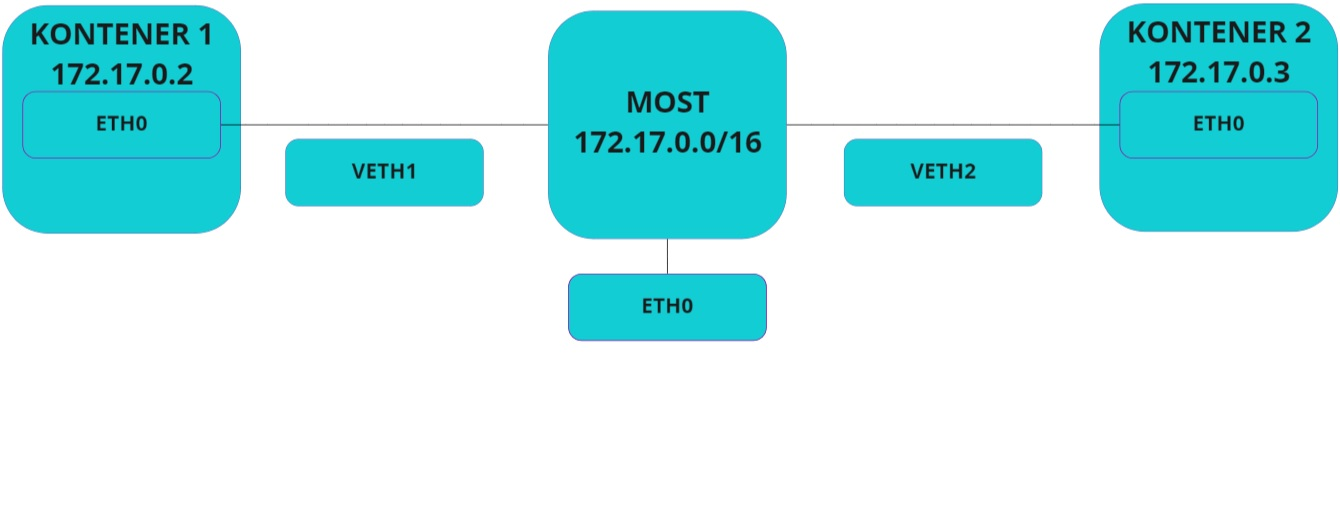
\includegraphics[width=1\textwidth]{container_networking.jpg}
  \caption{Łączność sieciowa w środowisku skonteneryzowanym. Opracowanie własne}
  \label{fig:container-networking}
\end{figure}

Platforma docker domyślnie tworzy most należący do podsieci 172.17.0.0/16.

Każdy kontener może uruchamiać procesy, które będą nasłuchiwać żądań na ustalonych portach.
Przestrzenie nazw posiadają oddzielne zestawy portów, dzięki czemu w każdej z nich może
zostać uruchomiony proces nasłuchujący przykładowo na porcie 80. Mapowanie portów w środowisku
kontenerów polega na skojarzeniu portów udostępnianych przez maszynę, na której uruchomione sobą
kontenery, z portami udostępnianymi przez przestrzenie nazw. Poniższy fragment przedstawia 
mapowanie między portem 80 udostępnianym przez przestrzeń nazw, w której uruchomiono mikrousługę ADS, 
a portem 8094 udostępnianym przez hosta:

\begin{lstlisting}
  ports:
      - "8094:80"
\end{lstlisting}

Dzięki temu usługi oferowane przez ten moduł danych są dostępne
pod adresem \textit{http://localhost:8094}.

\subsection{Ciągła integracja}

Podstawowym wymaganiem, które należy spełnić przy tworzeniu rozbudowanych systemów 
informatycznych, jest przechowywanie rozwijanego oprogramowania przy pomocy wybranego 
narzędzia kontroli wersji, takiego jak Git \cite{git2022}. Dane są zapisywane w folderze zwanym 
repozytorium. Zadaniem takiego narzędzia jest śledzenie wprowadzonych zmian 
oprogramowania i zapisywanie ich w historii repozytorium. Zapewnia to wiele 
korzyści, z których najważniejsze to:

\begin{itemize} % lista nienumerowana
    \item Podgląd zmian wprowadzonych przez każdego dewelopera
    \item Możliwość powrotu do poprzedniej wersji w przypadku, gdy wprowadzone zmiany 
    były przyczyną błędów w działaniu systemu
\end{itemize}

Głównym celem ciągłej integracji (ang. \textit{continuous integration}) jest regularne włączanie 
bieżących zmian w kodzie do głównego repozytorium i każdorazowa weryfikacja 
wprowadzonych zmian poprzez utworzenie nowego zbioru plików wykonywalnych 
i przeprowadzenie na nich testów jednostkowych. Zaletą tego podejścia jest fakt, że 
po wysłaniu przez programistę zmian do repozytorium głównego, reszta czynności 
wykonywana jest automatycznie przez serwer ciągłej integracji, bez ingerencji 
człowieka. Dodatkowo programista otrzymuje szybką odpowiedź zwrotną w razie 
wystąpienia błędów.
Aby wykorzystać potencjał ciągłej integracji, należy zwrócić uwagę na następujące 
punkty: 

\begin{itemize} % lista nienumerowana
    \item Częste i regularne wysyłanie kodu do głównego repozytorium w celu weryfikacji 
    integracji nowych zmian z resztą kodu, przynajmniej raz dziennie 
    \item Zapewnienie testów jednostkowych sprawdzających poprawność zachowania systemu. 
    Może się zdarzyć, że wprowadzone zmiany będą zgodne pod względem 
    składni, jednak nie oznacza to, że serwis będzie prawidłowo spełniał swoje 
    funkcje 
    \item Nadanie wysokiego priorytetu naprawieniu kodu, który nie integruje się z 
    dotychczasowym kodem w repozytorium. Odkładanie poprawy na później może spowodować 
    spiętrzenie się kolejnych błędów, co w konsekwencji bardziej spowolni wdrażanie 
    nowych funkcji
\end{itemize}

W trakcie tworzenia pracy wykorzystano platformę do ciągłej integracji i wdrażania 
o nazwie Github Actions. Pozwala ona na automatyzację tworzenia nowych wersji 
oprogramowania, testowania oraz wdrażania. Kolejne powtórzenia przepływów pracy 
(ang. \textit{workflow}) są wykonywane na maszynach wirtualnych oferowanych przez 
GitHub, zwanych pracownikami (ang. \textit{worker}). W zależności od potrzeby na maszynach 
zainstalowany jest odpowiedni system operacyjny spośród sytrybucji 
linux-owych, Windowsa oraz macOS.

\textit{GitHub Action} jest przepływem pracy, który może zostać wywołany zawsze wtedy, gdy 
zostanie zarejestrowane nowe zdarzenie dotyczące wykorzystywanego repozytorium. 
Przykładem zdarzenia jest wprowadzenie nowych zmian do repozytorium lub utworzenie 
żądania typu \textit{pull request}. \textit{GitHub Action} składa się z jednej lub większej liczby 
zadań (ang. \textit{job}), które mogą zostać wykonane jedno po drugim lub równolegle. Z kolei 
każde zadanie składa się z jednego lub większej liczby kroków (ang. \textit{step}), z których 
każde może wykonać własnoręcznie utworzony skrypt lub akcję (ang. \textit{action}), będącą 
rozszerzeniem umożliwiającym uproszczenie całego przepływu pracy.

Przykładowy przepływ pracy utworzony na potrzeby projektu wykonuje następujące zadania:

\begin{itemize} % lista nienumerowana
    \item Wybiera odpowiednią gałąź z repozytorium, na której zostały wprowadzone 
    nowe zmiany
    \item Instaluje wymagane oprogramowanie niezbędne do wykonania wszystkich 
    pozostałych zadań, takie jak środowisko .NET 5.0
    \item Uruchamia testy jednostkowe i integracyjne
    \item Tworzy nową wersję obrazu sprawdzonego mikroserwisu
    \item Wypycha obraz do rejestru kontenerów
\end{itemize}

Warto szczegółowo prześledzić poszczególne kroki danego przepływu.

\begin{lstlisting}
jobs:
  docker-build-and-push:
    runs-on: ubuntu-latest
    steps:
    - name: Checkout
      uses: actions/checkout@v2
      with:
        fetch-depth: 0
\end{lstlisting}

Powyższy wyciąg deklaruje nowe zadanie oraz pierwszy z kroków, który wybierze 
odpowiędnią gałąź z repozytorium. Parametr runs-on wskazuje jaki rodzaj systemu 
operacyjnego powinien zostać wykorzystany.

\begin{lstlisting}
on:
  workflow_dispatch: # allows to trigger workflow on demand
  push:
    branches: 
      - main
      - develop
    paths:
      - src/DagAir_Facilities/**
\end{lstlisting}

GitHub Actions oferuje rozbudowany system do określania warunków, które muszą być 
spełnione, aby uruchomić przepływ pracy. Powyższy wyciąg przedstawia fragment, który 
określa, że przepływ ma być uruchomiony gdy:

\begin{itemize} % lista nienumerowana
    \item Użytkownik manualnie uruchomi przepływ za pomocą interfejsu graficznego
    \item Zostaną wprowadzone nowe zmiany na gałęzi main lub develop oraz zmiany będą 
    się znajdować w katalogu \textit{src/DagAir\_Facilities/}
\end{itemize}

\begin{lstlisting}
- name: Build & Test
    shell: bash
    run: ./build.sh TestProject 
        --ProjectName facilities --verbosity verbose
\end{lstlisting}

Powyższy krok wykonuje skrypt uruchamiający testy jednostkowe oraz integracyjne.

\begin{lstlisting}
- name: Set image names & main tags
run: |
  appImageName="${{ env.
    CONTAINER_REGISTRY }}/${{ env.SERVICE_NAME }}"
  migrationsApplierImageName=
    "${{ env.CONTAINER_REGISTRY }}/${{ env.
    MIGRATIONS_APPLIER_NAME }}"
  echo "APP_IMAGE_NAME=$appImageName" >> $GITHUB_ENV
  echo "MIGRATIONS_APPLIER_IMAGE_NAME
    =$migrationsApplierImageName" 
    >> $GITHUB_ENV

  version="${{ steps.gitversion.outputs
    .nugetVersionV2 }}-${{ steps.gitversion
    .outputs.shortSha }}"

  if [ ${{ steps.gitversion.outputs
    .commitsSinceVersionSource }} -gt 0 ]; then
  version="${{ steps.gitversion.outputs
    .escapedBranchName }}-$version"
  fi

  echo "APP_IMAGE_TAG=${appImageName}:$version" 
    >> $GITHUB_ENV
  echo "MIGRATIONS_APPLIER_IMAGE_TAG=
  ${migrationsApplierImageName}:$version" \
  >> $GITHUB_ENV
\end{lstlisting}

Powyższy krok generuje nazwę oraz tag nowego obrazu testowanego mikroserwisu. Na nazwę 
obrazu składa się nazwa repozytorium obrazów oraz nazwa mikroserwisu. Numer wersji 
obrazu za każdym razem powinien być unikalny, ponadto powinien wskazywać, która z 
wersji obrazu jest najnowsza. Wobec tego na wersję składa się nazwa gałęzi 
repozytorium, nazwa utworzonej paczki Nuget-owej oraz krótki unikalny numer przypisany 
do migawki (ang. \textit{commit}), która spowodowała uruchomienie przepływu.

\begin{lstlisting}
- name: Docker login
  uses: docker/login-action@v1
  with:
    registry: ${{ env.CONTAINER_REGISTRY }}
    username: ${{ secrets.AZURE_CR_USERNAME }}
    password: ${{ secrets.AZURE_CR_PASSWORD }}

- name: Docker push images
  run: |
    docker push ${{ env.APP_IMAGE_NAME }} --all-tags
    docker push ${{ env.MIGRATIONS_APPLIER_IMAGE_NAME }} 
        --all-tags
\end{lstlisting}

Na samym końcu gotowy obraz zostaje wypchnięty do repozytorium obrazów. W tym celu 
używana jest komenda \textit{docker push}. Aby zakończyła się pomyślnie, należało 
w poprzednim kroku zalogować się do repozytorium, wykorzystując nazwę repozytorium obrazów oraz 
danych uwierzytelniających, przechowywanych w bezpieczny sposób za pomocą Github 
Secrets.

\subsection{Ciągłe dostarczanie}

W trakcie prac nad systemem wykorzystano metodykę ciągłego dostarczania, która polega na tym, że kod 
przechodzi przez kolejne fazy testowania, gdzie za każdym razem jest weryfikowana jego poprawność pod 
względem prawidłowego funkcjonowania. 

Na początku przeprowadzane są szybkie testy jednostkowe sprawdzające punktowo poprawność 
poszczególnych funkcji. Jeśli zostaną wykonane pomyślnie, przechodzi się do następnej fazy 
testowania uwzględniające wolniejsze testy, które sprawdzają zachowanie wielu serwisów między 
sobą. Po upewnieniu się, że ta faza została wykonana pomyślnie, system jest weryfikowany przez 
klienta, który zlecał jego wykonanie (tzw. \textit{user acceptance testing}). Jeśli funkcjonalność zgadza się z 
oczekiwaniami klienta, całość jest jeszcze testowana pod kątem wydajności, po czym zostaje 
wdrożona na etap produkcyjny.

Zgodnie z założeniami metodyki, programiści powinni otrzymywać
wiadomości zwrotne dotyczące statusu kolejnych wersji 
oprogramowania w kolejnych fazach testowania. Wprowadzenie takiego potoku potrafi znacznie
poprawić ocenę jakości kodu, ponadto skrócić czas między wdrożeniem kolejnych wersji systemu.

\subsection{Kubernetes}
Sekcja opisuje zasady działania oraz sposób wykorzystania narzędzia Kubernetes.
Podrozdziały 9.4.1 - 9.4.2 przedstawiają poszczególne komponenty, z których
składa się narzędzie. Podrozdział 9.4.3 przybliża sposób komunikacji
kontenerów znajdujących się w klastrze ze sobą oraz ze światem zewnętrznym.

Kubernetes jest platformą do orkiestracji kontenerów automatyzującą procesy manualne 
związane z wdrażaniem, zarządzaniem oraz skalowaniem skonteneryzowanych aplikacji. 
Jest to oprogramowanie typu open-source, początkowo rozwijane przez firmę Google
\cite{kubernetes2022}.

W przeszłości, organizacje uruchamiały aplikacje na fizycznych serwerach. W momencie 
gdy wiele aplikacji działało w ramach jednego serwera, dochodziło do 
sytuacji, w których jedna z nich zajmowała większość zasobów, przez co inne 
nie działały optymalnie. Jednym z rozwiązań było uruchomienie każdej 
z aplikacji na innym fizycznym serwerze. Jednak w takim wypadku konsekwencjami były 
wysokie koszty utrzymania infrastruktury. Innym możliwym rozwiązaniem było wprowadzenie 
wirtualizacji, które przyczyniło się do bardziej zrównoważonego zarządzania zasobami. 
Efektem ubocznym było jednak wprowadzanie dużego nakładu zasobów potrzebnych na 
uruchomienie samej maszyny wirtualnej, ponieważ każda z maszyn instalowała na początku 
własny system operacyjny.

Najlepszym obecnie rozwiązaniem jest wykorzystanie kontenerów. Zawierają zestaw 
podobnych cech do maszyn wirtualnych z tą różnicą, że nie wymagają osobnego systemu 
operacyjnego. Każdy z kontenerów może współdzielić jeden system operacyjny z 
innymi, co znacznie obniża wymagania dotyczące zasobów. Podobnie do maszyn 
wirtualnych posiadają własny system plików, zasoby obliczeniowe, pamięć. Jednak nie 
zależą od infrastruktury, na której są uruchamiane, co czyni je przenośnymi wśród 
różnych dystrybucji danego systemu.

Kontenery stały się popularne ze względu na szereg zalet:

\begin{itemize} % lista nienumerowana
    \item Utworzenie obrazów następuje szybciej w porównaniu do maszyn wirtualnych
    \item Obrazy zostają utworzone na etapie budowania nowej wersji systemu zamiast na etapie wdrażania
    \item Niezależnie od środowiska działają w dokładnie ten sam sposób
    \item Mogą być uruchomione praktycznie na każdym systemie i dystrybucji
    \item Cechują się wysoką efektywnością wykorzystania zasobów
\end{itemize}

Rysunek \ref{fig:deployment-types}. przedstawia różnice między uruchomieniem aplikacji w sposób 
tradycyjny, przy użyciu maszyn wirtualnych oraz kontenerów.

\begin{figure}[h]
    \centering
    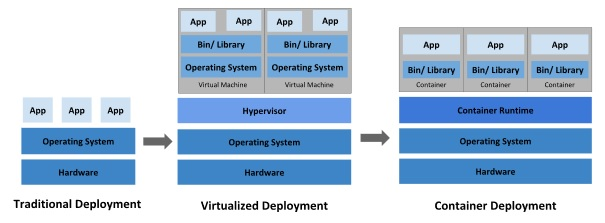
\includegraphics[width=1\textwidth]{deployment_types.jpg}
    \caption{Porównanie różnych metod uruchamiania aplikacji. Źródło: \cite{kubernetes2022}}
    \label{fig:deployment-types}
\end{figure}

Zalety Kubernetesa to przede wszystkim:

\begin{itemize} % lista nienumerowana
    \item Orkiestracja kontenerów między różnymi serwerami
    \item Efektywniejsze wykorzystanie zasobów
    \item Łatwe skalowanie skonteneryzowanych aplikacji 
    \item Zarządzanie serwisami w sposób deklaratywny
    \item Kontrola stanu aplikacji, automatyczne restartowanie kontenerów, 
    autoskalowanie
\end{itemize}

Zbiór hostów wykorzystywanych do uruchomienia na nich systemu zwany jest klastrem. Na 
każdym z hostów, zwanych węzłami, można uruchomić instancje gotowych obrazów. Każdy 
z klastrów posiada przynajmniej jeden węzeł.

Cyklem życiowym każdego kontenera zarządza płaszczyzna sterowania (ang. \textit{control 
plane}), która wystawia API oraz interfejsy umożliwiające ich wdrażanie i zarządzanie. 
Komponenty płaszczyzny mogą być uruchomione na każdej maszynie w klastrze, chociaż 
zazwyczaj określa się jedną maszynę, tzw. gospodarza (ang. \textit{master}), na której znajdują się 
wszystkie komponenty.

\subsubsection{Komponenty płaszczyzny sterowania}

W tabeli \ref{tab:komponenty-sterowania} zostały opisane komponenty składające się na całość płaszczyzny 
sterowania.
\newpage

\begin{xltabular}{1\textwidth} { 
  | >{\raggedright\arraybackslash}c 
  | >{\raggedright\arraybackslash}X | }
  \caption{Komponenty płaszczyzny sterowania} \label{tab:komponenty-sterowania}\\
  \hline
 Nazwa komoponentu & Opis \\
 \hline
 Kube-apiserver & Interfejs pozwalający na interakcję z płaszczyzną sterowania. 
 Weryfikuje i konfiguruje dane dla obiektów takich jak serwisy czy kontrolery 
 replikacji \\
 \hline
 Etcd & Spójny i wysoce dostępny magazyn par klucz-wartość używany przez Kubernetesa 
 jako miejsce do przechowywania wszystkich danych ważnych z punktu widzenia klastra.  \\
 \hline
 Kube-scheduler & Regularnie sprawdza czy został utworzony nowy zestaw 
 kontenerów, któremu nie został jeszcze przypisany węzeł. W takim przypadku wybiera 
 on maszynę, na której kontenery mają być uruchomione. Przy wyborze pod uwagę brane są 
 takie czynniki jak wymagane zasoby, ograniczenia sprzętowe lub programowe \\
 \hline
 Kube-controller-manager & Komponent odpowiedzialny za uruchamianie kontrolerów, które 
 monitorują oraz zmieniają stan klastra korzystając z API serwera \\
 \hline
 Cloud-controller-manager & Element, który wbudowuje logikę związaną z konkretną 
 chmurą, w której tworzone są klastry. Pozwala połączyć dany klaster z API dostawcy 
 chmury oraz oddziela komponenty, które oddziałują z chmurą od komponentów, które 
 oddziałują tylko z klastrem. Jest to komponent, który występuje tylko w przypadku 
 stawiania kontenerów w chmurze. Jeśli Kubernetes działa np. w prywatnym środowisku 
 na jednym komputerze, wtedy klaster nie posiada tego elementu \\
 \hline
\end{xltabular}

Istnieje kilka rodzajów kontrolerów:

\begin{itemize}
    \item Kontroler węzłów (ang. \textit{node controller}) - odpowiedzialny za wykrycie oraz 
    odpowiednią reakcję w przypadku, gdy jeden z węzłów ulega awarii lub staje się 
    niedostępny
    \item Kontroler prac (ang. \textit{job controller}) - nasłuchuje na pojawienie się obiektów 
    pracy (job objects) reprezentujących zadania, a następnie tworzy zbiór (pod) który 
    te zadania wykona
    \item Kontroler punktów końcowych - zarządza obiektami punktów końcowych (serwisy 
    oraz zbiory (ang. \textit{pods}))
    \item Kontroler kont oraz tokenów - tworzy domyślne konta oraz tokeny dostępu do 
    API dla nowych przestrzeni nazw
\end{itemize}

\subsubsection{Komponenty węzła}

W tabeli \ref{tab:komponenty-wezla} opisano komponenty, które działają na każdym węźle w Kubernetesie.

\begin{xltabular}{1\textwidth} { 
  | >{\raggedright\arraybackslash}c 
  | >{\raggedright\arraybackslash}X | }
  \caption{Komponenty węzła} \label{tab:komponenty-wezla}\\
  \hline
 Nazwa komponentu & Opis \\
 \hline
 Kubelet & Agent, którego rolą jest upewnienie się, że kontenery są uruchomione 
 w zbiorze (pods). Przyjmuje zestaw specyfikacji zbiorów i zapewnia, że wszystkie 
 kontenery podane w specyfikacji działają i są sprawne. Kubelet nie zarządza 
 kontenerami, które nie zostały utworzone przez Kubernetesa. \\
 \hline
 Kube-proxy & Proxy sieciowe, które implementuje część serwisu pozwalającego wystawić 
 aplikację do świata zewnętrznego. Jego zadaniem jest utrzymanie reguł sieciowych 
 w zarządzanych węzłach. Te reguły pozwalają na komunikację między różnymi zbiorami 
 wewnątrz lub na zewnątrz klastra.  \\
 \hline
 Container runtime & Oprogramowanie odpowiedzialne za uruchamianie kontenerów. 
 Kubernetes wspiera wiele możliwych runtime-ów, m. in. Docker, containerd, CRI-O. \\
 \hline
 Pod & Grupa złożona z jednego lub większej liczby kontenerów, wdrożona na tym samym 
 węźle. Wszystkie kontenery z grupy współdzielą adres IP oraz przydzielone zasoby. \\
 \hline
 Replication controller & Narzędzie do kontroli liczby kopii danego poda, które powinny 
 być w danej chwili uruchomione \\
 \hline
\end{xltabular}

Płaszczyzna sterowania przyjmuje komendy od administratora klastra, po czym przekazuje 
je do podległych serwerów. Komendy przyjmowane są za pomocą interfejsu 
konsolowego, zwanego \textit{kubectl}. Dobrą praktyką jest utworzenie plików deklarujących 
pożądany stan, w jakim powinien znajdować się klaster. Przykładowa deklaracja znajduje 
się poniżej.

\begin{lstlisting}
apiVersion: apps/v1
kind: Deployment
metadata:
  name: web-admin-app
  labels:
    app: web-admin-app
    tier: backend
spec:
  replicas: 2
  selector:
    matchLabels:
      app: admin-application-service
  template:
    metadata:
      labels:
        app: admin-application-service
        tier: backend
    spec:
      containers:
      - name: admin-application-service
        image: admin-application-service:develop-latest
        env:
        - name: ASPNETCORE_ENVIRONMENT
          value: "Kubernetes"
        imagePullPolicy: Always
        ports:
        - containerPort: 80
\end{lstlisting}

Jest to deklaracja typu \textit{Deployment}, która powinna zawierać następujące parametry:

\begin{itemize} % lista nienumerowana
    \item Wersja wykorzystywanego API
    \item Typ deklaracji
    \item Nazwa deklaracji
    \item Specyfikacja przedstawiająca pożądany stan, w jakim powinien znajdować się 
    klaster. W tym przypadku deklaruje się, że w klastrze powinny działać dwie 
    instancje obrazu mikrousługi aplikacyjnej dla administratorów, które powinny 
    nasłuchiwać na żądania na porcie 80
\end{itemize}

Komenda \textit{kubectl apply -f deployment.yml} umożliwia zaaplikowanie deklaracji.

Płaszczyzna sterowania jest odpowiedzialna za to, by stan klastra odpowiadał 
deklaracji. W konsekwencji zostaną utworzone dwa osobne pody, z których każdy otrzyma 
unikalny prywatny adres IP wewnątrz klastra. Od tej pory do każdej instancji można 
się odwołać, wykorzystując jej adres IP oraz numer portu.

Należy wziąć pod uwagę, że pody nie są trwałymi zasobami. Mogą być tworzone i usuwane 
w sposób dynamiczny. Za każdym razem pod otrzymuje nowy adres IP, który może się 
różnić od poprzednich. Prowadzi to do problemów przy komunikacji między 
mikroserwisami, ponieważ nie wiedzą, że wymagany mikroserwis nie jest już osiągalny pod 
dotychczasowym adresem.

Rozwiązaniem tego zagadnienia jest wprowadzenie tzw. serwisu (ang. \textit{service}). Jest to abstrakcyjny 
obiekt, który definiuje zbiór pod-ów oraz reguły umożliwiające do nich dostęp. 
Serwisowi nadawany jest unikalny adres IP, pod który mogą odwoływać się mikroserwisy. 
W dalszym ciągu pod-y będą dynamicznie tworzone i usuwane, jednak w tym wypadku będą 
one ciągle dostępne pod adresem IP serwisu.

Przykładem jest poniższa deklaracja:

\begin{lstlisting}
apiVersion: v1
kind: Service
metadata:
  name: admin-application-service
  labels:
    app: admin-application-service
    tier: backend
spec:
  selector:
    app: admin-application-service
  type: LoadBalancer
  ports:
  - port: 8085
    targetPort: 80
    protocol: TCP
    name: http 
\end{lstlisting}

Jest to deklaracja typu \textit{Service}, która powinna zawierać następujące parametry:

\begin{itemize} % lista nienumerowana
    \item Wersja wykorzystywanego API
    \item Typ deklaracji
    \item Nazwa deklaracji
    \item Selektor. Od niego zależy, które pod-y zostaną dołączone do zbioru
    \item Typ publikacji
    \item Porty
\end{itemize}

Wyróżnia się trzy główne typy publikacji serwisu:

\begin{itemize} % lista nienumerowana
    \item ClusterIP - typ domyślny. Przydziela serwisowi wewnętrzny adres IP 
    w klastrze, przez co serwis jest dostępny jedynie dla innych obiektów uruchomionych 
    wewnątrz klastra
    \item NodePort - przydziela serwisowi statyczny numer portu na każdym węźle 
    w klastrze. Dzięki temu serwis jest dostępny dla obiektów znajdujących się poza 
    klastrem i można się do niego dostać przy pomocy adresu IP węzła oraz statycznego 
    numeru portu
    \item LoadBalancer - przydziela serwisowi adres zewnętrzny przy użyciu load 
    balancer-a zapewnionego przez wykorzystywaną platformę chmurową
\end{itemize}

Dobrą praktyką jest utworzenie obiektu wejścia do klastra (ang. \textit{ingress}), który 
zarządza dostępem do klastra z zewnątrz. Typowo jest to obiekt API, który udostępnia 
ścieżki protokołu HTTP(S) prowadzące do serwisów znajdujących się wewnątrz klastra.

Przykład deklaracji znajduje się poniżej.

\begin{lstlisting}
apiVersion: networking.k8s.io/v1
kind: Ingress
metadata:
  name: example-ingress
  annotations:
    kubernetes.io/ingress.class: nginx
    nginx.ingress.kubernetes.io/ssl-redirect: "false"
    nginx.ingress.kubernetes.io/affinity: cookie
    nginx.ingress.kubernetes.io/session-cookie-hash: sha1
    nginx.ingress.kubernetes.io/session-cookie-name: 
        REALTIMESERVERID
    nginx.org/websocket-services: 
        "admin-application-service"
spec:
  tls:
    - hosts:
      - dagair.info
      secretName: ingress-cert
  rules:
    - host: dagair.info
      http:
        paths:
          - path: /adminapplication
            pathType: Prefix
            backend:
              service:
                name: web-admin-app
                port:
                  number: 8085
\end{lstlisting}

Jest to deklaracja typu \textit{Ingress}, która powinna zawierać następujące parametry:

\begin{itemize} % lista nienumerowana
    \item Wersja wykorzystywanego API
    \item Typ deklaracji
    \item Nazwa deklaracji
    \item Specyfikacja, która zawiera reguły związane z dostępem do poszczególnych 
    serwisów w klastrze. W tym przypadku aplikacja dla administratorów jest dostępna 
    pod adresem dagair.info/adminapplication
\end{itemize}

\subsubsection{Łączność sieciowa w środowisku Kubernetes}

Łączność sieciowa w środowisku Kubernetes w dużym stopniu pokrywa się z zasadami funkcjonowania
na platformie Docker, które zostały opisane w podrozdziale \ref{subsubection:lacznosc-sieciowa-docker}.
Wewnątrz hosta utworzone są odrębne przestrzenie nazw, połączone ze sobą mostem. Dodatkowym poziomem
abstrakcji są pody, wewnątrz których można uruchomić wiele kontenerów. Każdy pod otrzymuje unikalny adres
IP. Kontenery wewnątrz poda mogą komunikować się ze sobą za pomocą interfejsu \textit{loopback}.
W przypadku konieczności komunikacji z mikrousługami znajdującymi się na innych hostach pakiety
należy wysłać poprzez interfejs \textit{ETH0} hosta. 
Kubernetes oferuje serwis DNS pozwalający na translację nazw serwisów na adresy IP.

Rysunek \ref{fig:kubernetes-networking} przedstawia strukturę sieciową klastra.

\begin{figure}[h]
  \centering
  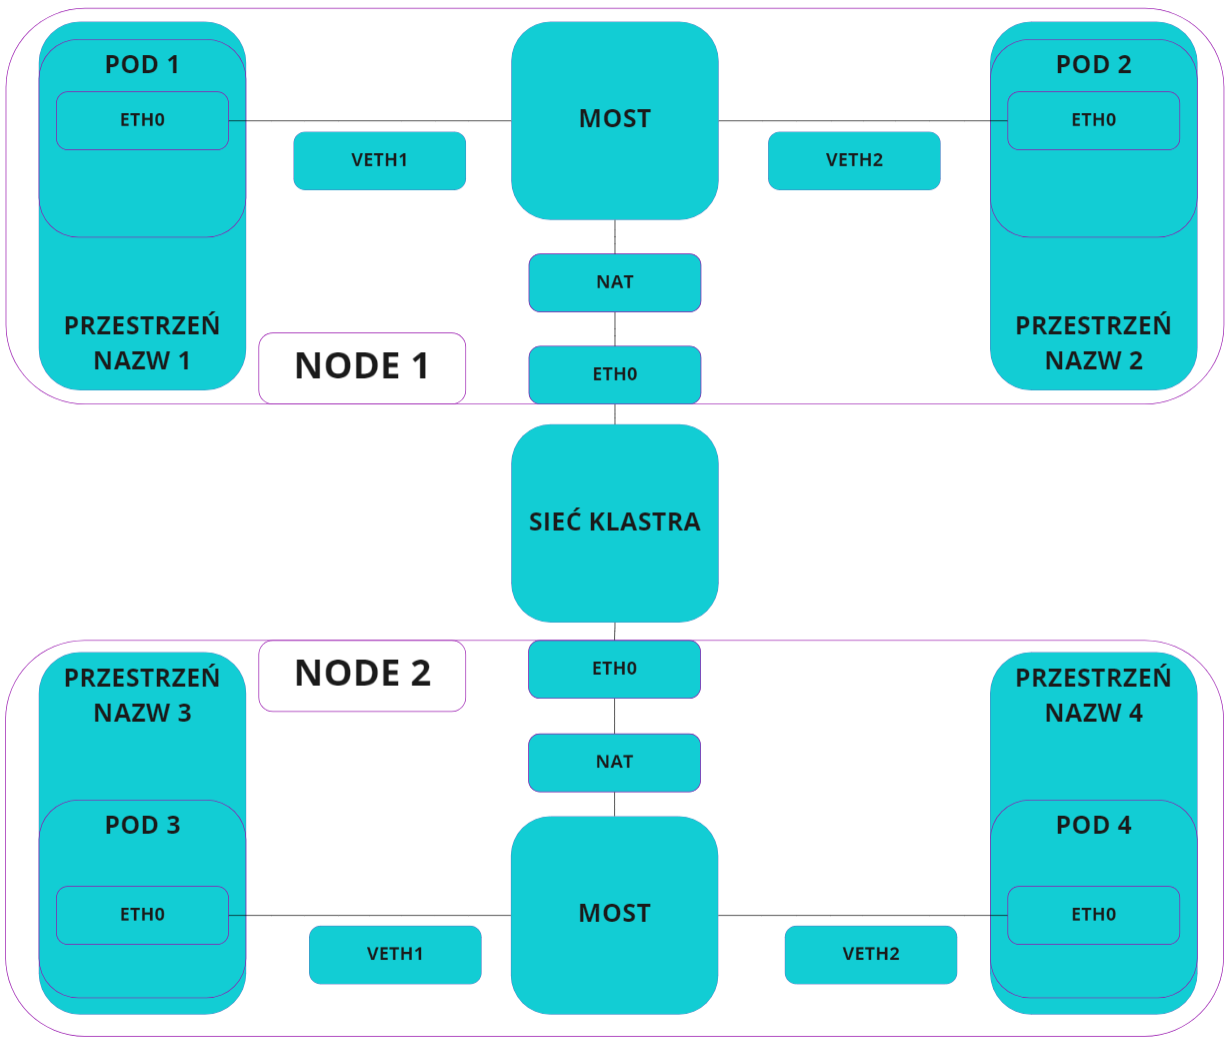
\includegraphics[width=0.9\textwidth]{kubernetes_networking.jpg}
  \caption{Łączność sieciowa w środowisku Kubernetes. Opracowanie własne}
  \label{fig:kubernetes-networking}
\end{figure}